\begin{frame}{\textbf{Abstract representation}}

Mapping plain abstracts to vector:

\begin{figure}
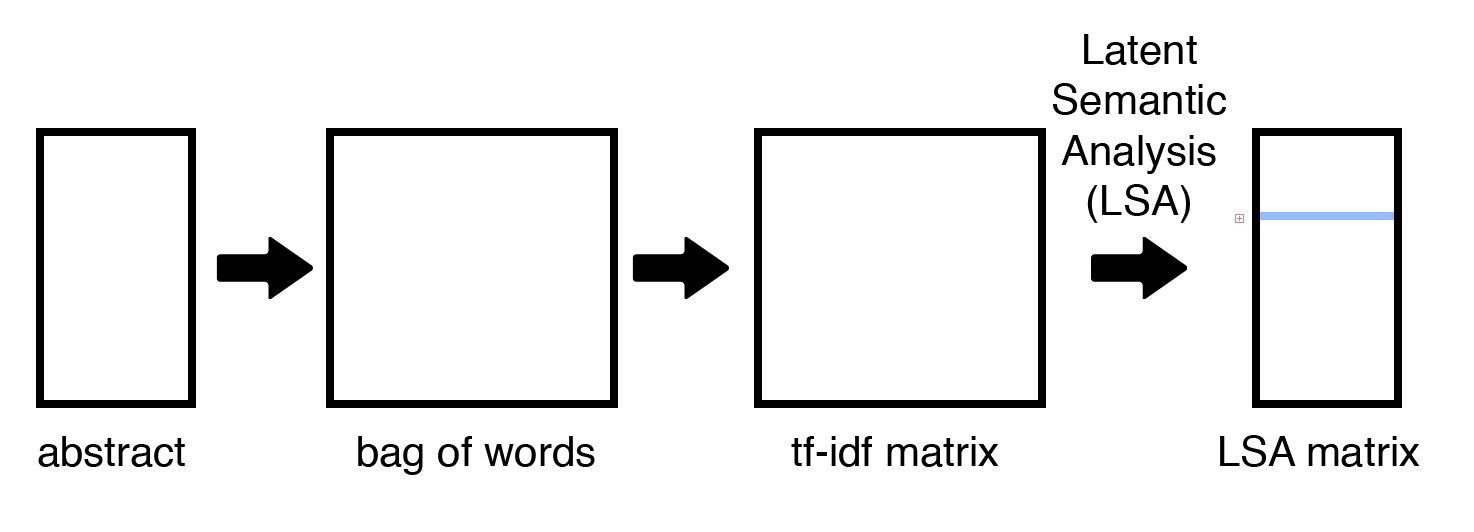
\includegraphics[width=2.5in]{images/algorithm_flow}\\
\tiny{Schematic of the workflow for converting abstracts into vector representations}
\end{figure}

Applying term frequency--inverse document frequency:
\begin{equation*}
\begin{split}
\text{tf-idf} &= \text{tf} \times \text{idf}\\
&=  (1 + \log f) \times \log \left( \frac{N}{ d } \right)
\end{split}
\end{equation*}

\begin{itemize}
\item $f$ is total number of words occurrence in each document
\item $d$ is number of documents where the term appears
\end{itemize}

\end{frame}


\begin{frame}{\textbf{Abstract representation}}

\begin{figure}
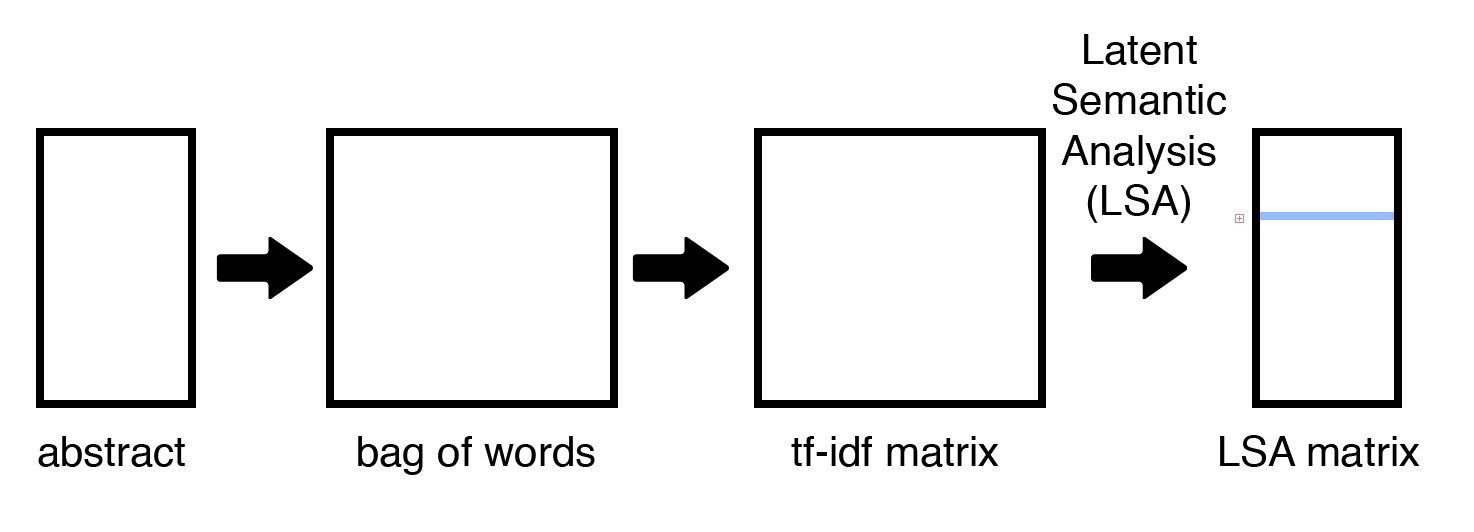
\includegraphics[width=2.5in]{images/algorithm_flow}\\
\tiny{Schematic of the workflow for converting abstracts into vector representations}
\end{figure}


\begin{itemize}
\item tf-idf vectorizer (weight more if words are distinctive of a document)
\item Latent Semantic Analysis - truncated SVD
\item $X = U \Sigma V^\intercal  \rightarrow X_{LSA} = U_r \Sigma_r V_r^\intercal$
\end{itemize}

\end{frame}


\begin{frame}{\textbf{t-SNE in 2D}}

\begin{figure}
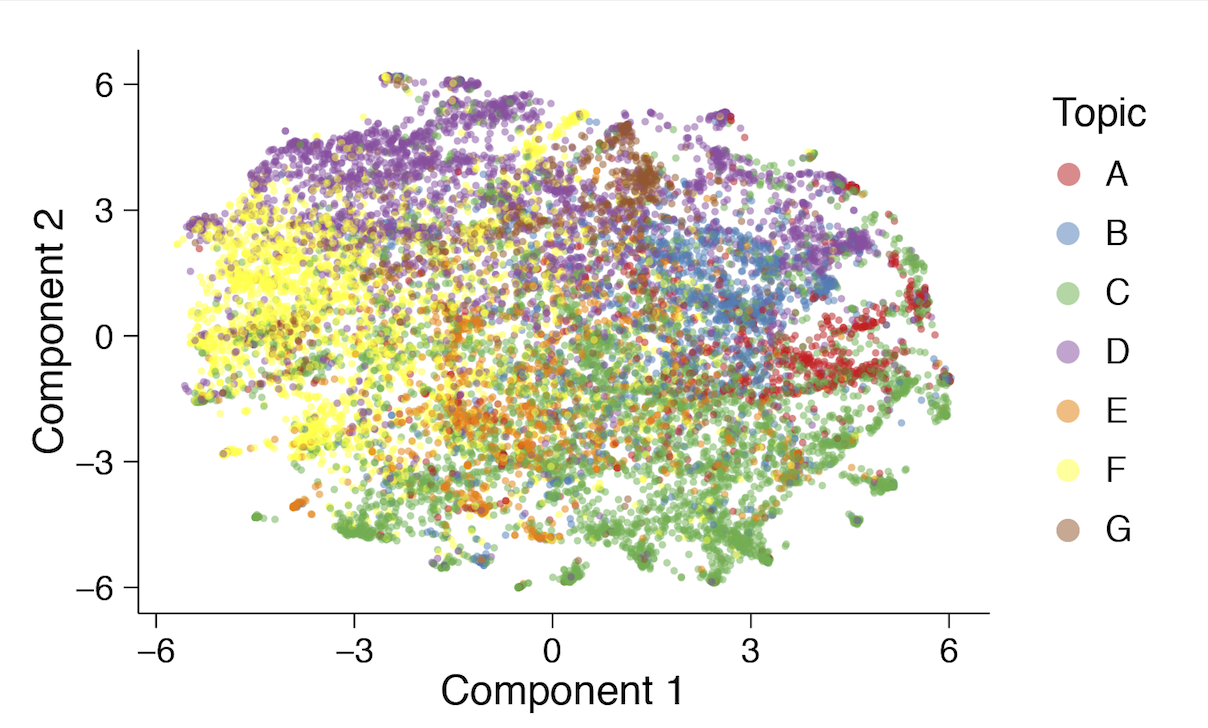
\includegraphics[width=2.5in]{images/tsne}\\
\tiny{Visualization of topics colored by human curated sessions using t-SNE on abstract vectors.}
\end{figure}

2D abstract topic representation is grouped by human curated topic
(see topic \href{https://github.com/titipata/science_concierge/wiki/Topic-in-SfN-2015}{\textbf{here}})

\end{frame}


\begin{frame}{\textbf{Abstract recommendation}}

We allow users to like/dislike abstracts and use nearest neighbor to provide $N$ closest abstracts ($\mathbf{x}_a$ = topic of abstract)

\begin{figure}
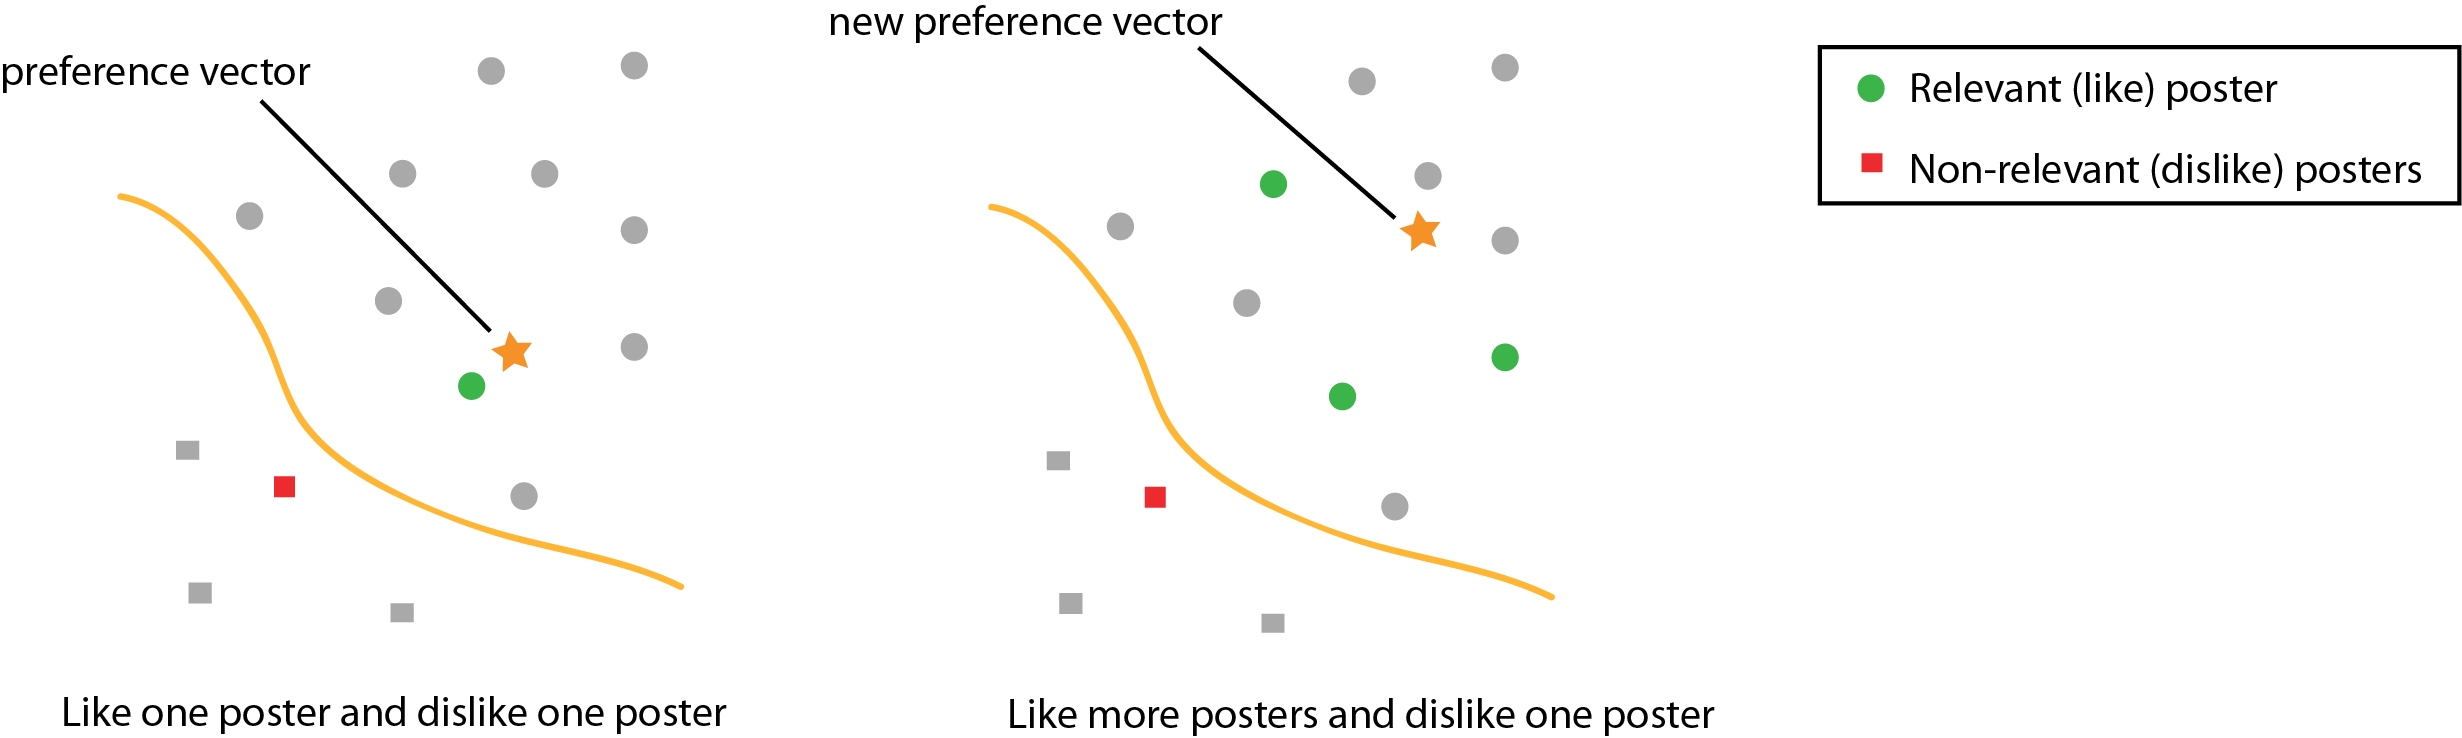
\includegraphics[width=2.2in]{images/like-dislike}\\
\tiny{Schematic of Modified Rocchio Algorithm algorithm (T Joachims, 1997)}
\end{figure}

\end{frame}


\begin{frame}{\textbf{Abstract recommendation}}

Original Rocchio Algorithm

\begin{equation*}
\mathbf{x}_a = \mathbf{x}_0 + (\alpha \cdot \frac{1}{\left| X_r \right|} \sum_{\mathbf{x}_j \in X_r} \mathbf{x}_j) - (\beta \cdot \frac{1}{\left| X_{nr} \right|} \sum_{\mathbf{x}_k \in X_{nr}} \mathbf{x}_k)
\end{equation*}

Modified Rocchio Algorithm

\begin{equation*}
\mathbf{x}_a = (\frac{\alpha}{\left| X_{nr} \right|} \cdot \sum_{\mathbf{x}_j \in X_r} \mathbf{x}_j) - (\frac{\beta}{\left| X_{nr} \right|} \cdot \sum_{\mathbf{x}_k \in X_{nr}} \mathbf{x}_k)
\end{equation*}

use less than 100 ms for each nearest neighbor assignment (for 50k posters)

\end{frame}
